\section{Test01: GPU vs CPU}
The results of this test are used as baseline for further optimizations. \\
Test configuration:
\begin{itemize}
  \item \textbf{CPU}: Intel(R) Core(TM) i7-4770K CPU @ 3.50GHz 
  \item \textbf{GPU}: NVIDIA Tesla K40c 
\end{itemize}
Implementations tested:
\begin{itemize}
  \item \textbf{legacy\_multifit\_cpu}: plain \textit{cms-sw} cpu code.
  \item \textbf{legacy\_multifit\_gpu}: plain gpu porting \textit{cms-sw} cpu code.
  \item \textbf{multifit\_cpu}: inplace fnnls cpu implementation.
  \item \textbf{multifit\_gpu}: inplace fnnls gpu implementation.
  \item \textbf{multifit\_cpu\_swap}: fnnls cpu implementation with swapping matrices.
  \item \textbf{multifit\_gpu\_swap}: fnnls gpu implementation with swapping matrices.
\end{itemize}
\begin{figure}[h]
  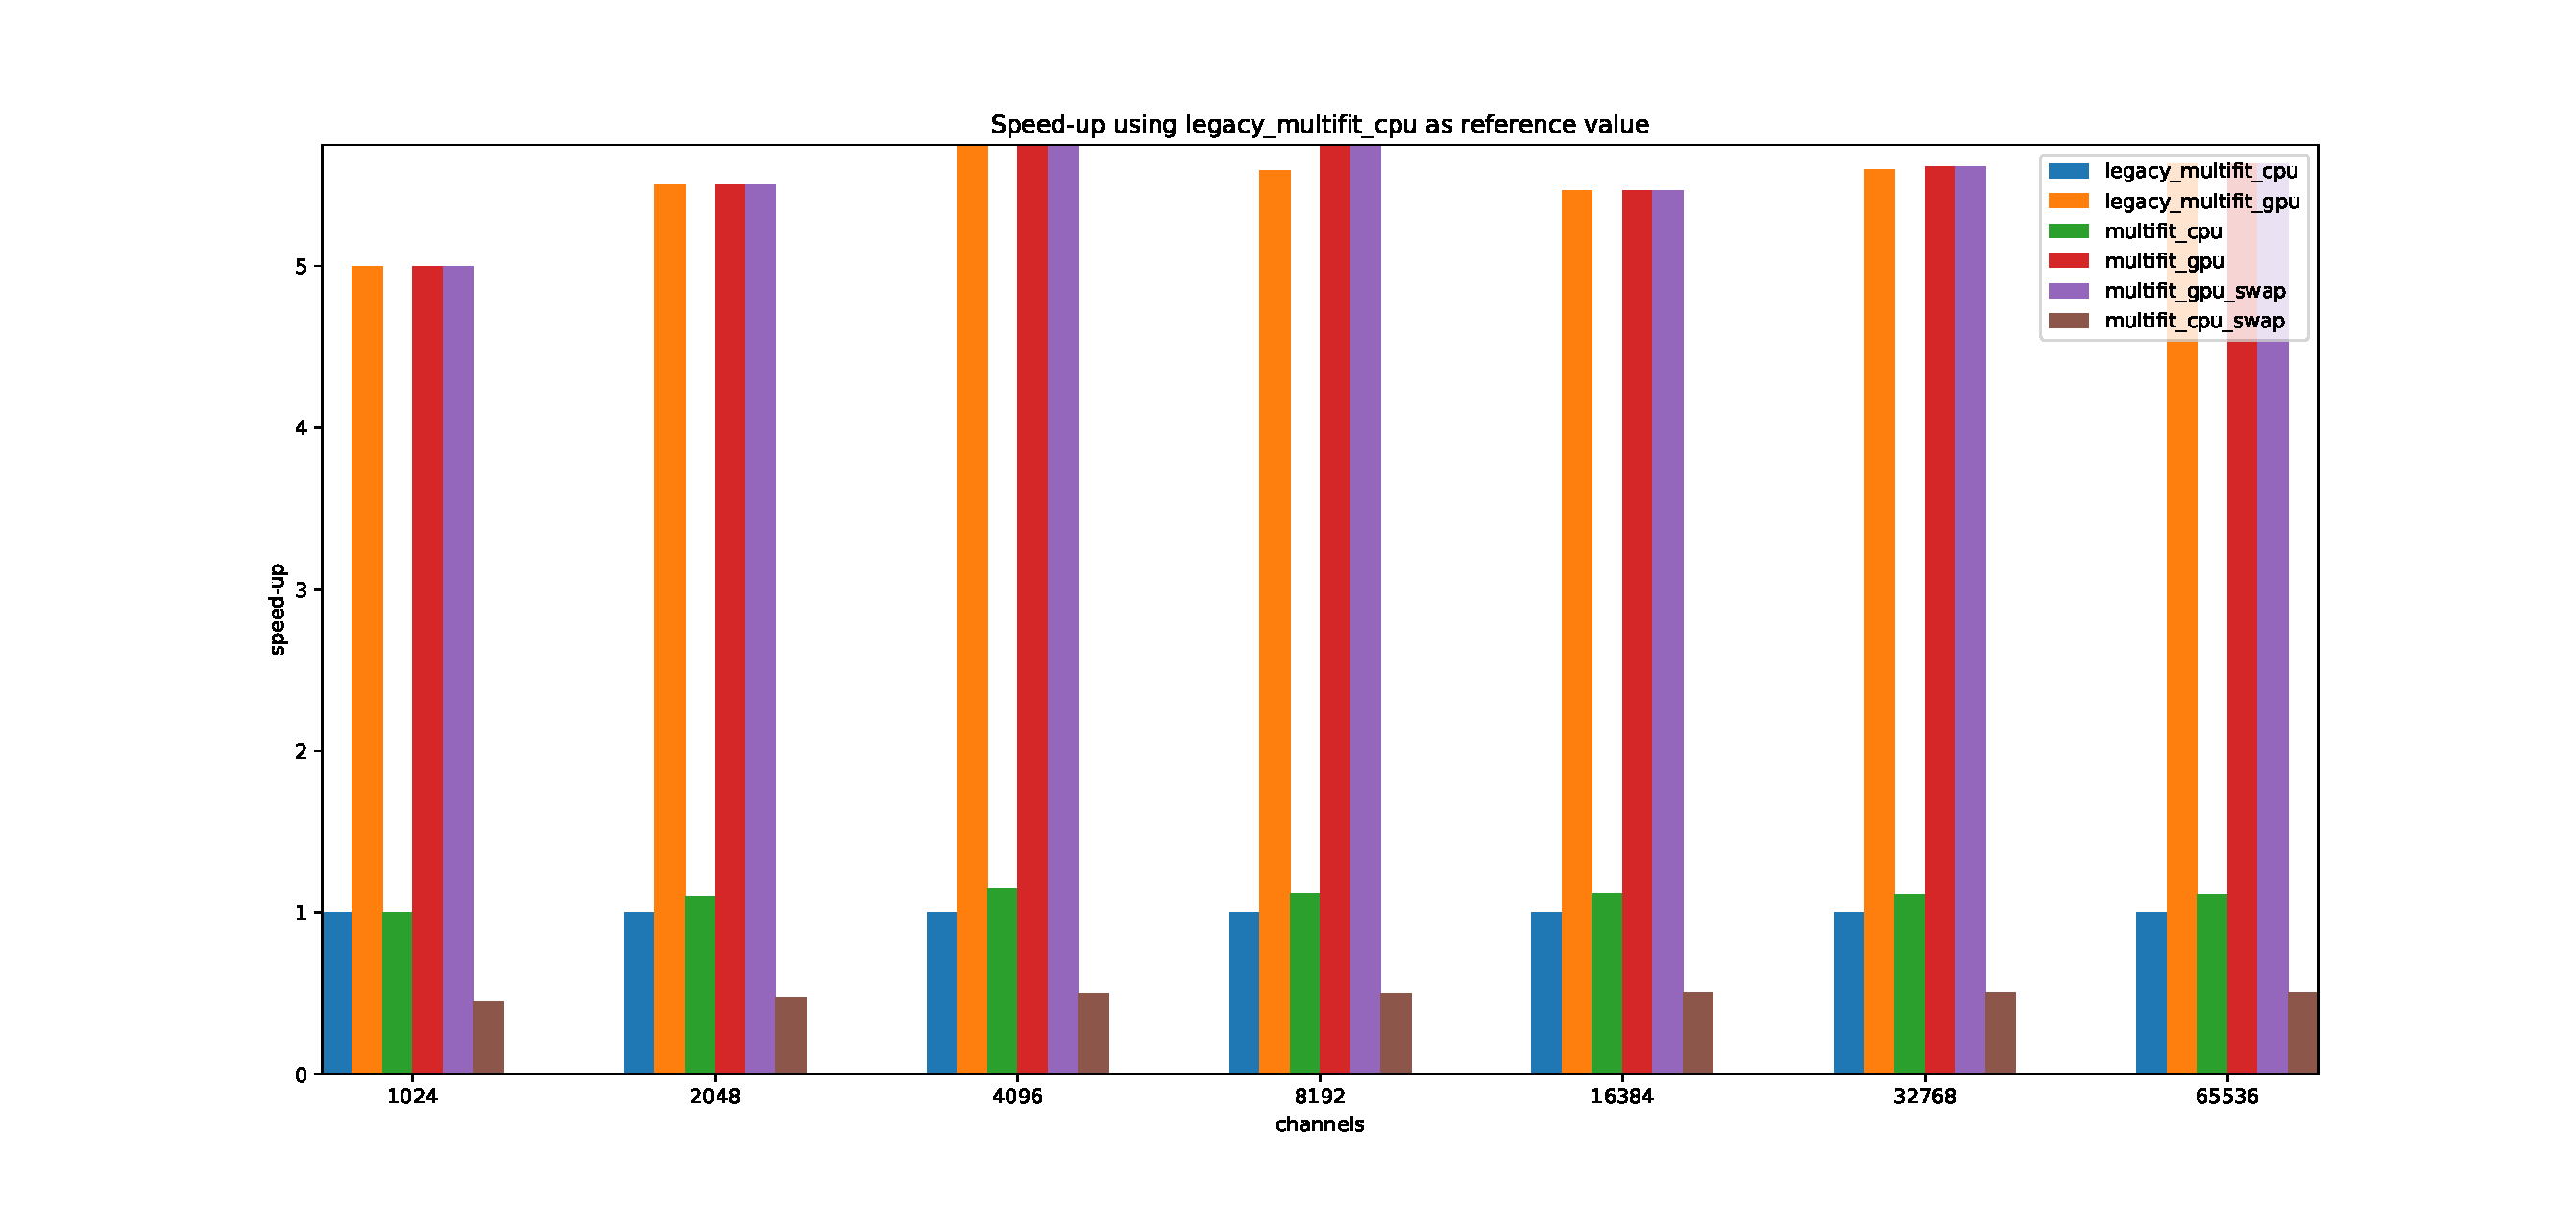
\includegraphics[width=\textwidth]{img/speedup}
  \caption{Speedup achieved with 10 iterations, higher is better}
  \label{img:speedup01}
\end{figure}
All the cpu implementations are single-threaded. With 64k channels the GPU version achieves a speedup of 7.2. It is interesting to notice that the unoptimized cpu version on gpu outperforms the other implementations.
\begin{figure}[H]
  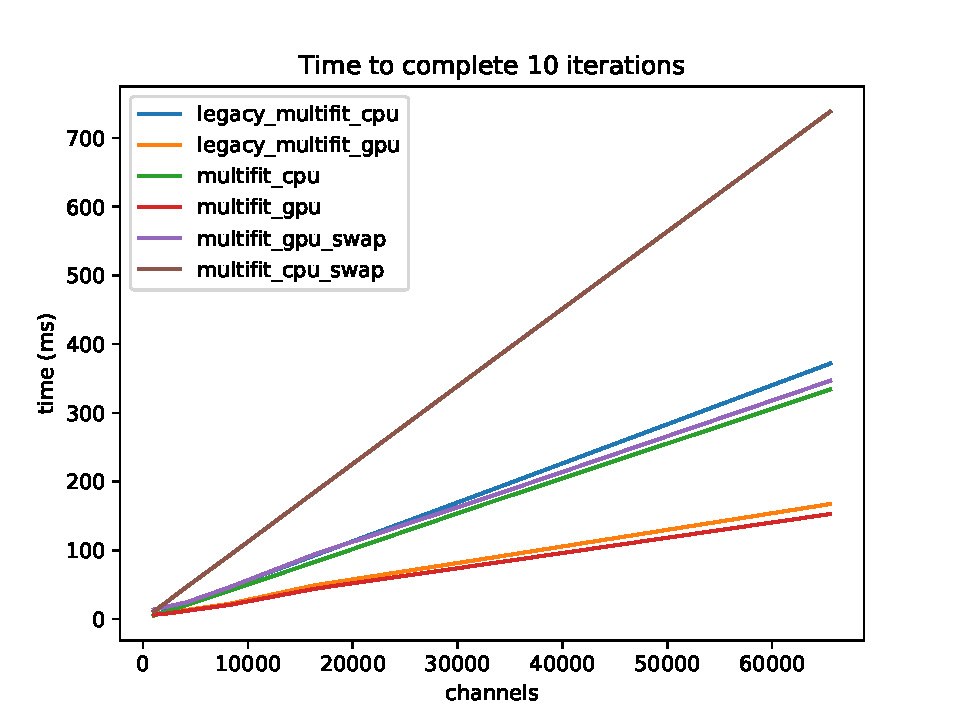
\includegraphics[width=.75\textwidth]{img/linscale}
  \caption{Time needed to complete 10 iterations, linear channel scale, lower is better}
  \label{img:linscale01}
\end{figure}
From \ref{img:speedup01} that the GPU performs seven times as fast with respect to the CPU. Other optimizations like loop unrolling and branch reduction give a performance gain about 20\% on CPU.
\begin{figure}[H]
  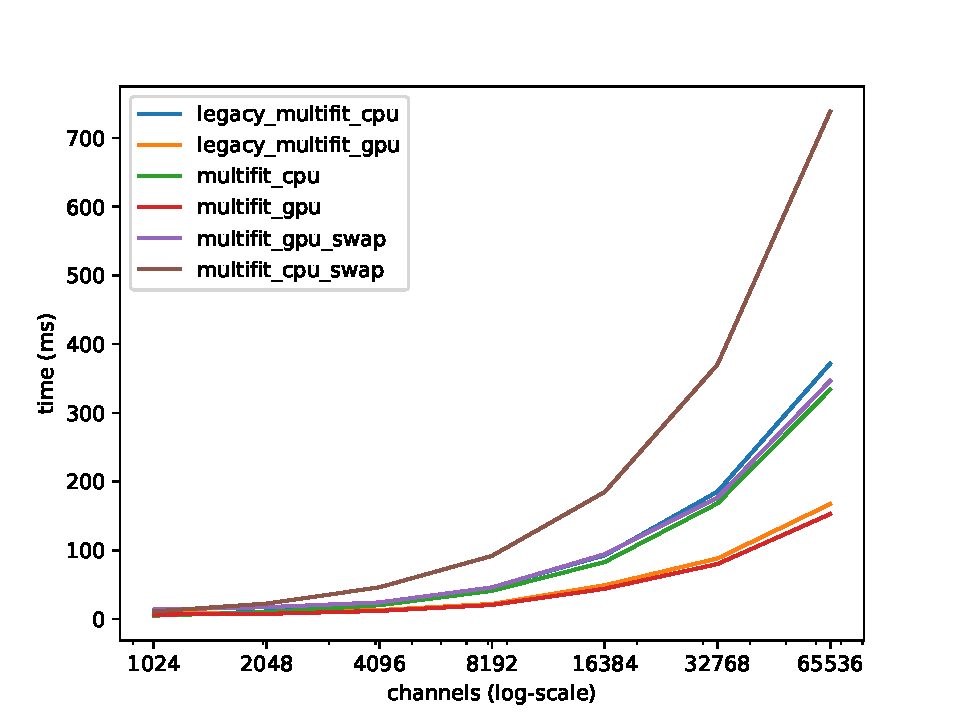
\includegraphics[width=.75\textwidth]{img/logscale}
  \caption{Time needed to complete 10 iterations, log channel scale, lower is better}
  \label{img:logscale01}
\end{figure}
From the plot present in \ref{img:linscale01} can be noted that, on the optimized CPU version, the time increases faster at the beginning but around 30000 channels there is a change of slope and the increase becomes sub-linear. On the GPU, the increase is always sub-linear with respect to the channels.
The plot in \ref{img:logscale01} makes more evident the difference between the different version of the algorithm. The GPU outperforms the CPU and it will be interesting to study what will happen if the number of channels increases even more.\\
\section{Test02: GPU vs CPU, Optimized Matrix multiplication}

\begin{figure}[h]
  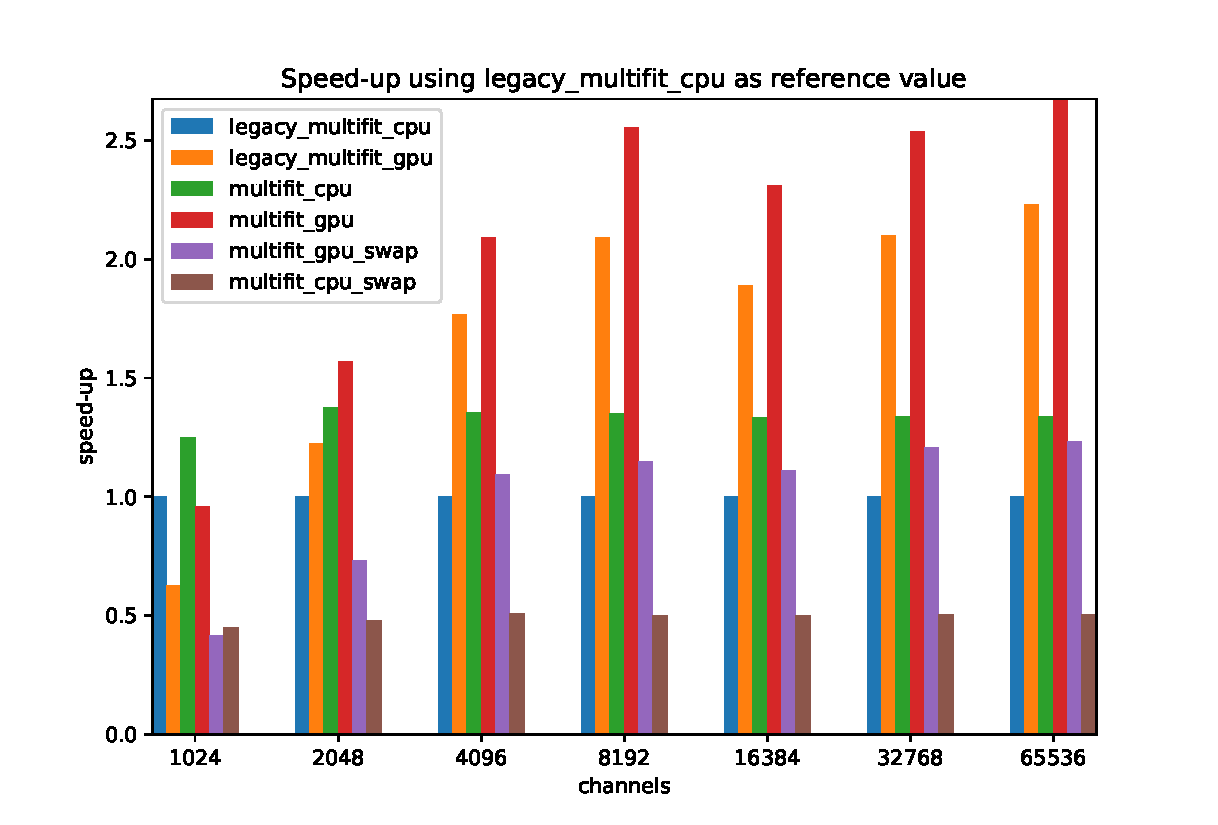
\includegraphics[width=\textwidth]{img/speedup02}
  \caption{Speedup achieved with 10 iterations, higher is better}
  \label{img:speedup02}
\end{figure}
All the cpu implementations are single-threaded. With 64k channels the GPU version achieves a speedup of 7.2. In this case, the swap and the optimized versions performs the same.
\begin{figure}[H]
  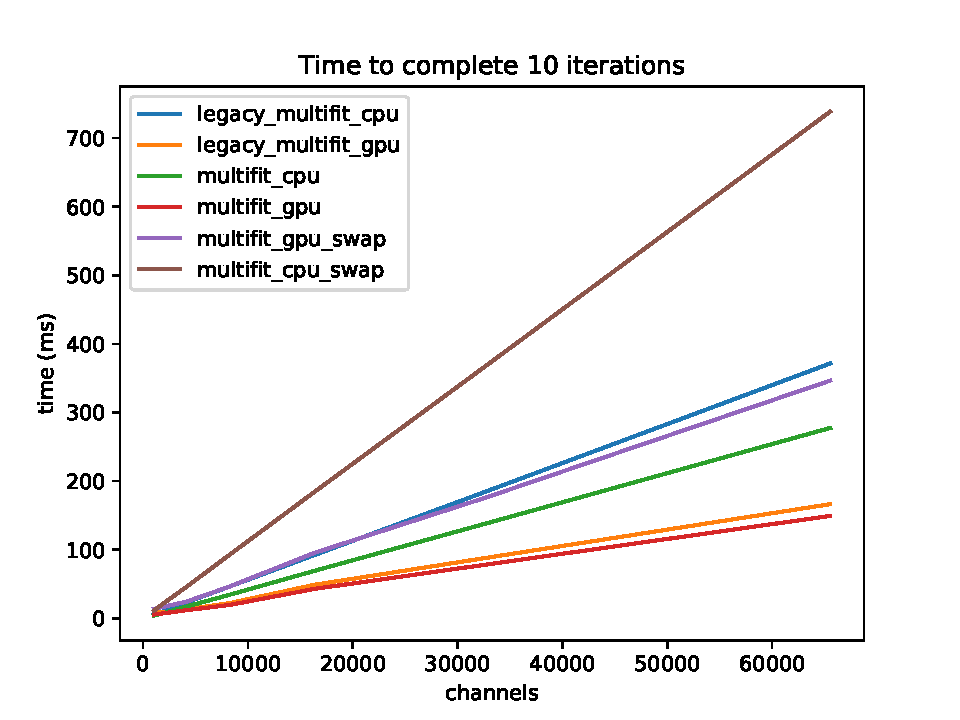
\includegraphics[width=.75\textwidth]{img/linscale02}
  \caption{Time needed to complete 10 iterations, linear channel scale, lower is better}
  \label{img:linscale02}
\end{figure}
From \ref{img:speedup01} that the GPU performs seven times as fast with respect to the CPU. The optimized CPU implementation in this case performs $40\%$ better than the legacy one. Also, the slope of the line generated legacy implementation is slightly super linear while the optimized version is sublinear. The GPU versions performs the same because in this test the GPU are underutilized.
\begin{figure}[H]
  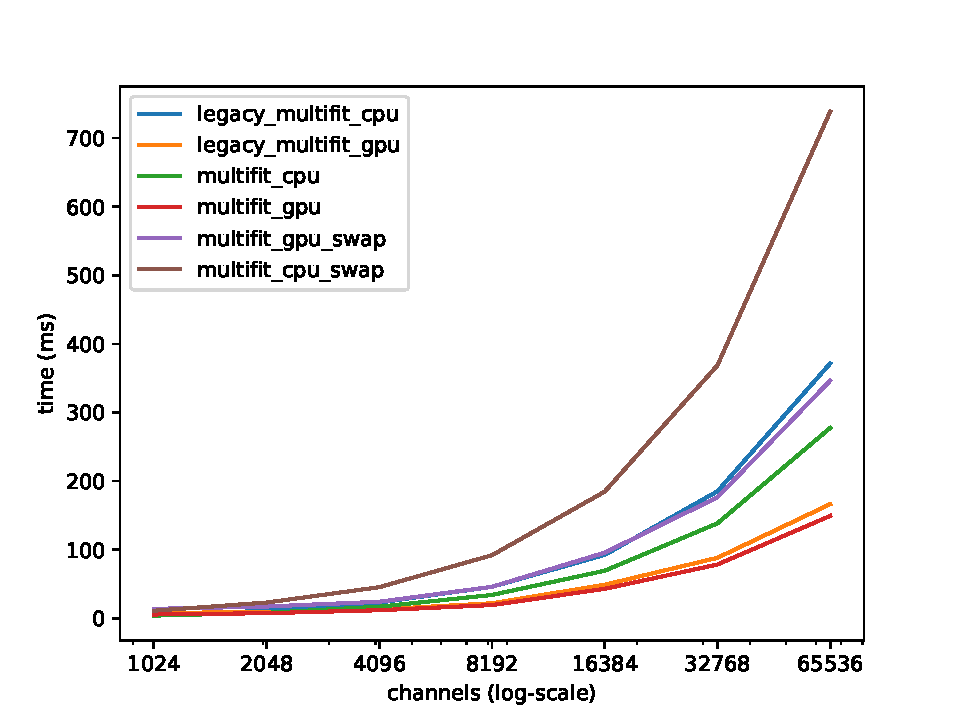
\includegraphics[width=.75\textwidth]{img/logscale02}
  \caption{Time needed to complete 10 iterations, log channel scale, lower is better}
  \label{img:logscale02}
\end{figure}